\subsection{Deployment view}
\par
Regarding the deployment, there are many quality to take into consideration. One of these is the scalability property: at the beginning 
TrackMe might only have few users, but once the usage is increasing more and more, the system must continue to work even if the 
requests from the users are huge. To achieve this quality of service, TrackMe needs the help of cloud database providers. These ones 
are specialized in the management of big database; and in this case the Share Data Service requires a huge database in order to store 
all the data collected from the users. Furthermore, since the services with the highest throughput are considered to be the spectator and the
data share one, these services will be deployed in a cluster: Docker can be used in order to provide images of the containerized environment. 
This, also, enhances scalability. 
\par
On the other side, services such as Account service, Individual Request Service and Group Request Service do not require so much power. 
Therefore, these services, at least in a first moment, are not thought to need a cluster: indeed, they will be deployed on the same physical 
machine, but with docker images in different virtual machines. 
In such a way each microservices has its own application server, while the database server can be shared among these services. 
However, with this approach, it will be easy to scale, in case it is necessary. \\
Note that the Spectator Service requires to save a good amount of data and 
the access might be frequent due to the requirement regarding the possibility to see all the positions of the runners during a race. 
Consequently, the Spectator Service has its own database server machine.
A further thing that is worth a comment is the fact that the router could be a cluster too, in order to avoid that it becomes the bottleneck 
of the architecture. 
\par
To access these microservices one needs to use the mobile application which has to be installed on an Android device.

\begin{figure}[H]
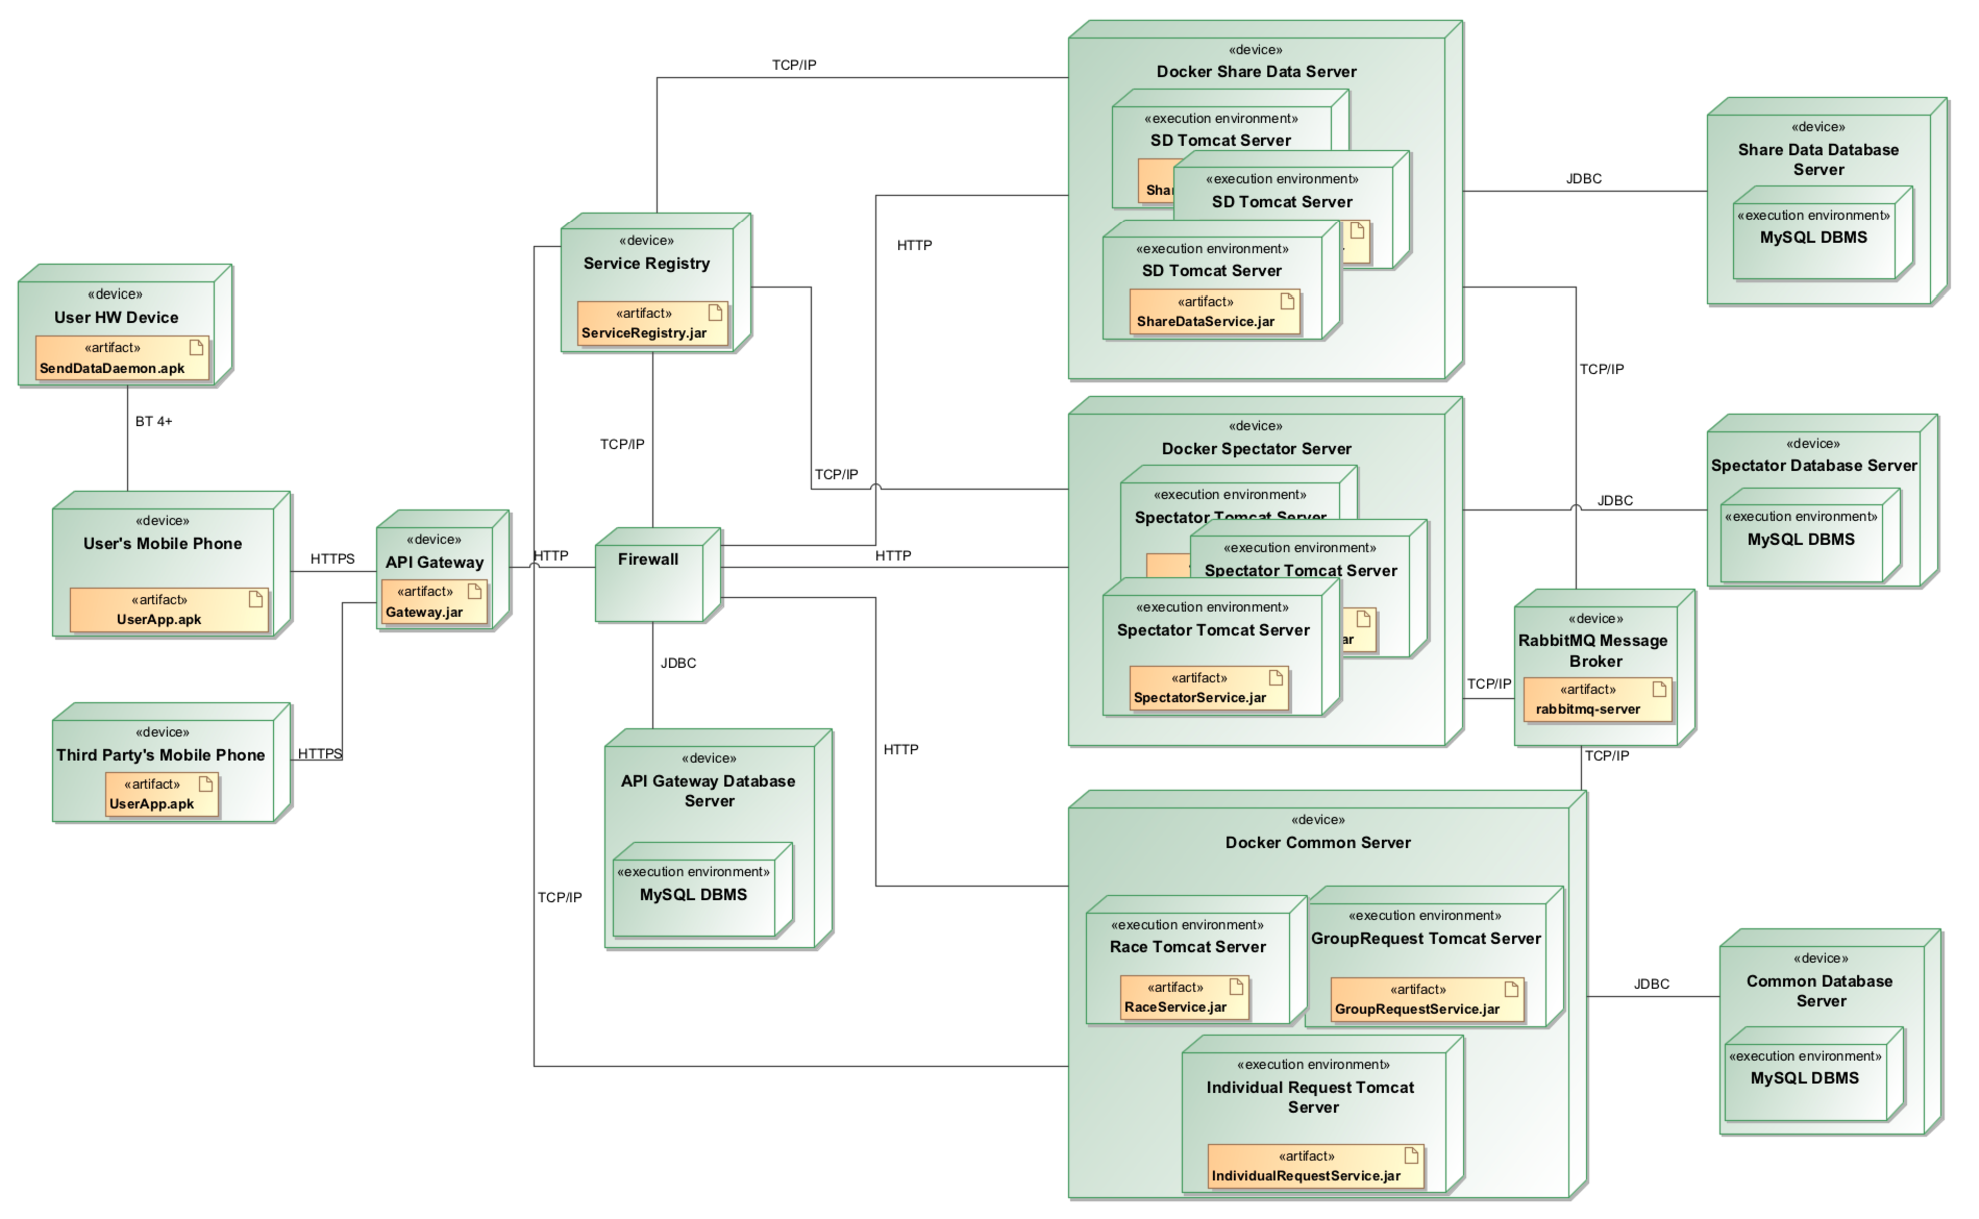
\includegraphics[width=\linewidth]{Images/deploymentdiagram.pdf}
\caption{ Deployment diagram with Archimate }
\label{fig:deployment}
\end{figure}

The deployment diagram represents the system to-be which is based on the microservices "reference architecture". Even if 
microservices offer the possibility to implement different services with different programming language or framework, what is simpler 
is to keep using the same environment. In this case, Tomcat application server and MySQL DBMS are strongly used. 